\documentclass[fleqn,10pt,french]{SelfArx} % Document font size and equations flushed left

\usepackage{lipsum} % Required to insert dummy text. To be removed otherwise
\usepackage[utf8]{inputenc} 

\setlength{\columnsep}{0.55cm} % Distance between the two columns of text
\setlength{\fboxrule}{0.75pt} % Width of the border around the abstract

\definecolor{color1}{RGB}{0,0,90} % Color of the article title and sections
\definecolor{color2}{RGB}{0,20,20} % Color of the boxes behind the abstract and headings

\usepackage{hyperref} 
\hypersetup{hidelinks,colorlinks,breaklinks=true,urlcolor=color2,citecolor=color1,linkcolor=color1,bookmarksopen=false,pdftitle={Title},pdfauthor={Author}}

\Archive{Projet d’INF 421} 
\PaperTitle{Résoudre de manière optimale le Rubik’s cube} 
\Authors{Kevin CHEN, Yuxiang LI} 
\affiliation{*\textbf{Code source}: https://github.com/lyx-x/Rubik} 
\Keywords{IDA* --- Pattern Database --- HashMap}
\newcommand{\keywordname}{Keywords}

%----------------------------------------------------------------------------------------
%	ABSTRACT
%----------------------------------------------------------------------------------------

\Abstract{TODO}

%----------------------------------------------------------------------------------------

\begin{document}

\flushbottom % Makes all text pages the same height

\maketitle % Print the title and abstract box

\renewcommand{\contentsname}{Table des matières}
\tableofcontents % Print the contents section

\thispagestyle{empty} % Removes page numbering from the first page

%----------------------------------------------------------------------------------------
%	ARTICLE CONTENTS
%----------------------------------------------------------------------------------------

\section{Analyse du sujet} % The \section*{} command stops section numbering

\lipsum[1-3] % Dummy text
 and some mathematics $\cos\pi=-1$ and $\alpha$ in the text\footnote{And some mathematics $\cos\pi=-1$ and $\alpha$ in the text.}.

%------------------------------------------------

\section{Implémentation}

\begin{figure*}[ht]\centering % Using \begin{figure*} makes the figure take up the entire width of the page
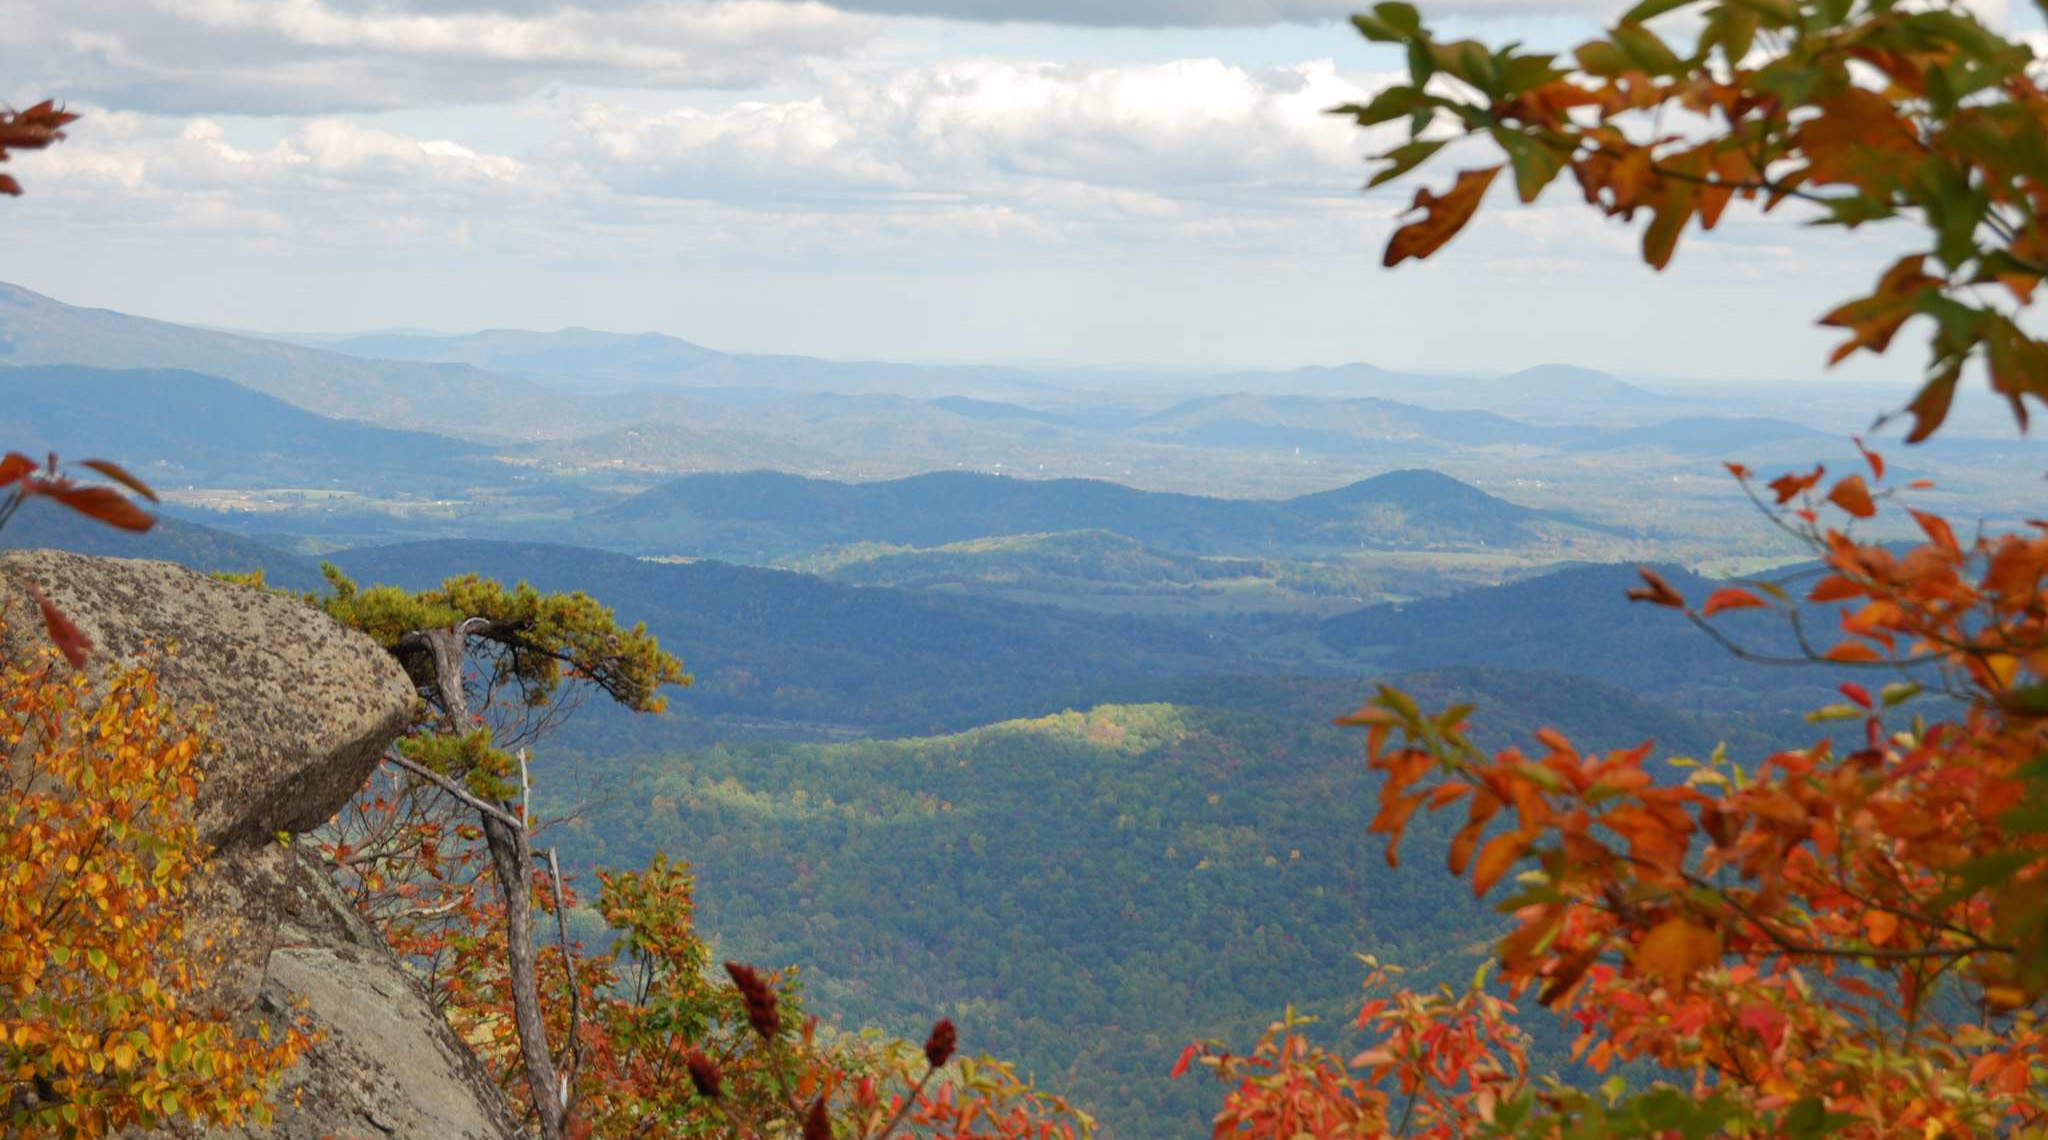
\includegraphics[width=\linewidth]{view}
\caption{Wide Picture}
\label{fig:view}
\end{figure*}

\lipsum[4] % Dummy text

\begin{equation}
\cos^3 \theta =\frac{1}{4}\cos\theta+\frac{3}{4}\cos 3\theta
\label{eq:refname2}
\end{equation}

\lipsum[5] % Dummy text

\begin{enumerate}[noitemsep] % [noitemsep] removes whitespace between the items for a compact look
\item First item in a list
\item Second item in a list
\item Third item in a list
\end{enumerate}

\subsection{Organisation du code}

\lipsum[6] % Dummy text

\paragraph{Paragraph} \lipsum[7] % Dummy text
\paragraph{Paragraph} \lipsum[8] % Dummy text

\subsection{Algorithmes de recherche}

\lipsum[9] % Dummy text

\begin{figure}[ht]\centering
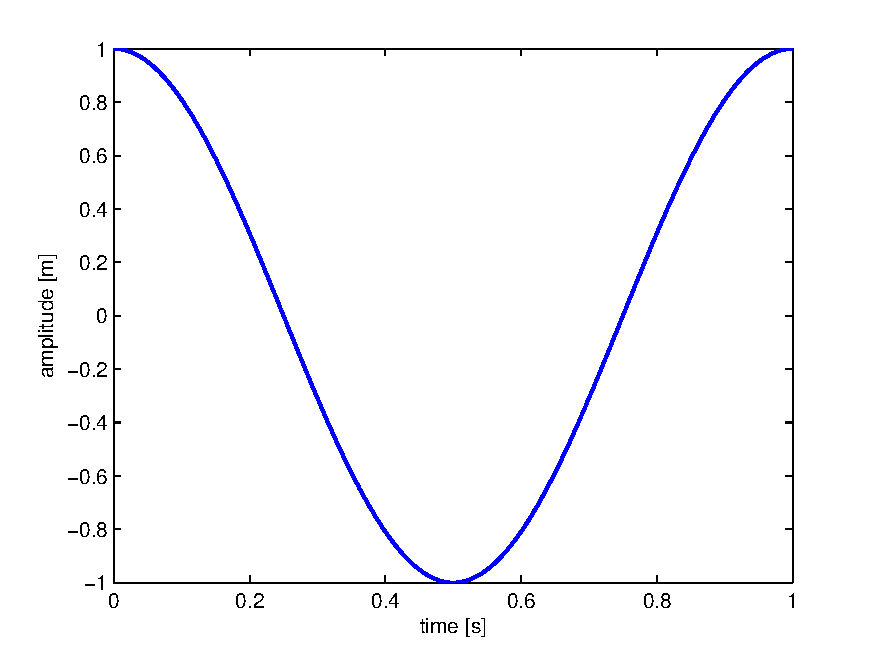
\includegraphics[width=\linewidth]{results}
\caption{In-text Picture}
\label{fig:results}
\end{figure}

Reference to Figure \ref{fig:results}.

%------------------------------------------------

\section{Résultats}

\lipsum[10] % Dummy text

\subsection{Tests}

\lipsum[11] % Dummy text

\subsection{Problèmes rencontrés}

\lipsum[11] % Dummy text

\begin{table}[hbt]
\caption{Table of Grades}
\centering
\begin{tabular}{llr}
\toprule
\multicolumn{2}{c}{Name} \\
\cmidrule(r){1-2}
First name & Last Name & Grade \\
\midrule
John & Doe & $7.5$ \\
Richard & Miles & $2$ \\
\bottomrule
\end{tabular}
\label{tab:label}
\end{table}

\subsubsection{Estimateur de la distance}

\lipsum[12] % Dummy text

\subsubsection{HashCode}

\lipsum[12] % Dummy text

\subsubsection{Opération du fichier}

\lipsum[12] % Dummy text

\begin{description}
\item[Word] Definition
\item[Concept] Explanation
\item[Idea] Text
\end{description}

\subsubsection{Pattern database}

\lipsum[13] % Dummy text

\subsubsection{Taille de HashMap}

\lipsum[13] % Dummy text

\begin{itemize}[noitemsep] % [noitemsep] removes whitespace between the items for a compact look
\item First item in a list
\item Second item in a list
\item Third item in a list
\end{itemize}

\subsection{Comparaison et conclusion}

\lipsum[15-23] % Dummy text

%------------------------------------------------
\phantomsection
\section*{Annexe} % The \section*{} command stops section numbering

\addcontentsline{toc}{section}{Annexe} % Adds this section to the table of contents

So long and thanks for all the fish \cite{Figueredo:2009dg}.

\end{document}